\chapter{Heatmap Regression}
\label{sec:heatmap}

% so far only binary classification \cite{George_2018}
% how to adapt to data stream? 

So far, this work has only dealt with the simplified problem of detecting one signal per sample, which can be treated as a binary-classification task. It remains to adapt this approach to a proper GW search. Such a search processes a data stream of arbitrary length and returns multiple GW candidates along with some confidence measure and their time location in that data.

% CNN Binary classifier + sliding window + postprocessing \cite{Sch_fer_2023}
% works for short LIGO-like signals where a small window suffices
% we need large receptive fields to capture waveforms fully ~1min
% but for large ET event rates the classifier will (almost) always spit out true
% final output becomes meaningless

One simple approach, followed by the models in \cite{Sch_fer_2023} for example, utilizes overlapping sliding windows of $\pazocal{O}(\SI{1}{\second})$. The already trained binary classifier assigns each window a score, resulting in a \enquote{probability} time series in $[0,1]$. Such a time series will be referred to as a \emph{heatmap} from now on. From this heatmap, a number of post-processing steps yield multiple GW candidates.

This approach is suitable for second-generation detector conditions, where signals are short. However in ET, waveforms are longer and thus, larger input sizes are required of $\approx\SI{1}{\minute}$. Further, ET's increased event rate means that these long-duration windows are almost always contaminated by some amount of signals. For example, a $\SI{64}{\second}$ sample will contain the merger of at least one signal with a probability $\approx\SI{87}{\percent}$ (see Fig.~\ref{fig:data_simulation:poisson}). Therefore, employing the classifier that was trained in Ch.~\ref{sec:long_duration} over sliding $\SI{64}{\second}$ windows, will return mostly positive labels, making the final output useless.

This chapter compares two different approaches. One is similar to existing research \cite{PhysRevD.100.063015}, and will be called \emph{heatmap regression}. Here, instead of training a binary classifier separately beforehand, the network is trained directly to produce a heatmap for a given $\SI{64}{\second}$ sample. 

The other approach is novel and completely forgoes the heatmap output, which has to be post-processed later. This model is fully end-to-end, \emph{i.e.}, for a given sample, it directly outputs multiple GW candidates with a score and time location. This is an adaptation of the \emph{Detection Transformer} (DETR) \cite{10.1007/978-3-030-58452-8_13}, which was originally developed for a vision task and had to be modified to handle time series instead.

% other approach heatmap regression \cite{PhysRevD.100.063015}
% explain heatmap
% fully convolutional -> apply to data stream of arbitrary length
% again postprocess to yield number of GW candidates with score and time

% \cite{PhysRevD.100.063015} train with 8s samples containing one signal at most
% this work uses 64s samples because of increased signal length
% and possibly multiple signals per sample (adapt)

% compare one cnn and one transformer model 
% because multiple signals in one sample -> transformer helps maybe?
% helps for gw parameter estimation \cite{Papalini_2025}
% Since it has been seen that networks only focus 1s around merger, improvements may be small here


\section{Problem Setup}

% datasets

Two datasets are simulated. The training dataset comprises \SI{1}{\mega\nothing} samples and the test data is \SI{66}{\kilo\nothing} samples. Each sample is \SI{64}{\second} long and contains up to six signals. Their coalescence times are sampled uniformly over the sample duration. The number of signals per sample is drawn from a uniform integer distribution in $[0,6]$. Instead of evaluating the network over a continuous data stream, models are tested over the independent samples in the test dataset. 

% define task

For each sample, the task is to make multiple GW signal predictions. These are denoted $\{(\hat{c}_i,\hat{t}_i)\}_{i=1}^{m}$, where each prediction comprises a class score $\hat{c}$ and the signal coalescence time $\hat{t}$. The ground-truth signals are characterized by their coalescence time $\{t_i\}_{i=1}^{n}$. Time values are normalized to the sample length. (Note that the number of predictions $m$ and the number of ground-truth objects $n$ can differ.) 

When evaluating the performance of GW search algorithms, two metrics are of interest, the \emph{false-alarm rate} (FAR) and the \emph{detection ratio}. These are defined as,
\begin{equation}
	\text{FAR} = \frac{\text{FP}}{\text{Length of analyzed data}}, \quad \text{Detection ratio} = \frac{\text{TP}}{\text{Number of signals in that data}},
\end{equation}
where TP and FP are true and false positives respectively. GW searches usually aim for a low FAR to make confident detections. Matched filtering reaches FARs of \SI{1}{\per\month} to \SI{1}{\per\year}.

To calculate these values, it has to be considered in which case a prediction should be labeled true (TP) and in which case false (FP). It is straightforward to call a prediction TP if the class prediction exceeds a threshold, $\hat{c}>z$, and if the \emph{corresponding} ground-truth signal is sufficiently close, $|t-\hat{t}|\leq\SI{0.1}{\second}$. Else, the prediction is counted as a FP.
Varying the threshold $z\in[0,1]$ yields multiple operating points $(\text{FAR}(z), \text{Detection ratio}(z))$. These can be plotted as an operating characteristic, which is convenient for evaluating the performance of different models. (In fact, this characteristic is very similar to a ROC, as FPR and TPR are equivalent to FAR and the detection ratio in binary classification at least. This work will refrain from this terminology here, since the definition of FAR and of the detection ratio differs in this context.)

Now, for a given prediction, what exactly is the \enquote{corresponding} ground-truth signal? Simply taking the closest signal in time does not suffice as it can result in multiple predictions being assigned to the same signal. Instead, this task requires defining some one-to-one matching algorithm. Each signal should be assigned one prediction, and if there are more predictions than signals, $n<m$, the left-over predictions are labeled FP.

For this, the earlier approach could be adapted by iterating over all predictions and finding the closest signal, under the condition that this signal has not been matched yet. Then, if prediction and signal are close enough in time, the signal marked as matched going on. The problem here is, that predictions and signals are assigned independent of the predicted class score. For example, a prediction with low class score can be assigned to a ground-truth signal although a prediction with high class score is also nearby. This issue can be easily resolved by iterating over predictions based on their class score, starting with the highest. The whole scheme can be summarized as follows:
\setlist{nolistsep}
\begin{itemize}[noitemsep]
	\item All predictions below the threshold, $\hat{c}<z$, are noise predictions and can be disregarded.
	\item The remaining signal predictions are sorted by decreasing $\hat{c}$.
	\item For each prediction, the closest unmatched ground-truth signal is found.
	\item If $|t-\hat{t}|\leq\SI{0.1}{\second}$, the prediction counts as a TP and the signal is marked as matched.
	\item Otherwise, the prediction is a FP and the signal is \emph{not} marked as matched.
	\item Once there are no unmatched signals left, the remaining predictions are counted as FPs.
\end{itemize}

\section{Heatmap Construction and Post-Processing}

\begin{figure}
	\centering
	\makebox[\textwidth][c]{%
	\begin{subfigure}{7cm}
		\centering
		\makebox[\textwidth]{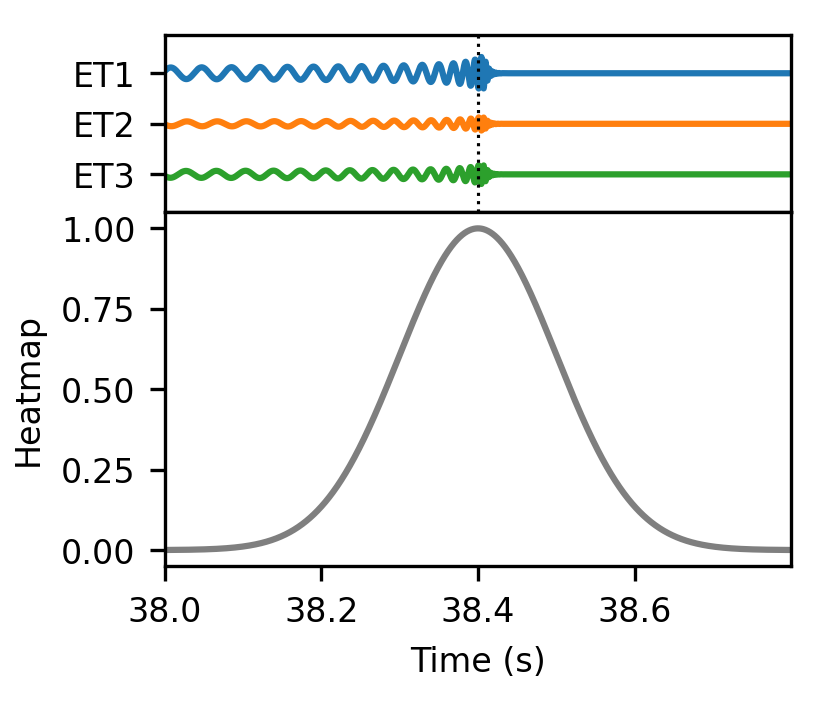
\includegraphics[width=7cm]{multiple_signal_detection/images/heatmap/heatmap_one_signal}}
		\caption{}
		\label{fig:heat:heatmap_one_signal}
	\end{subfigure}%
	\hspace{0.3cm}%
	\begin{subfigure}{9cm}
		\centering
		\makebox[\textwidth]{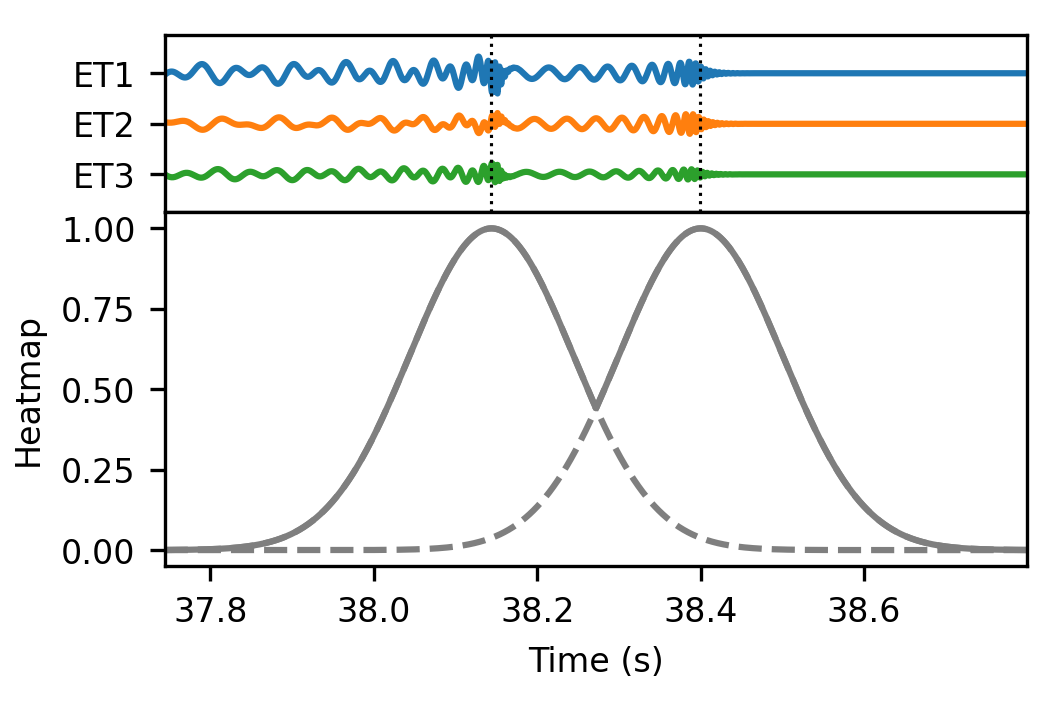
\includegraphics[width=9cm]{multiple_signal_detection/images/heatmap/heatmap_two_signals}}
		\caption{}
		\label{fig:heat:heatmap_two_signals}
	\end{subfigure}
	}
	\caption{}
\end{figure}

\begin{figure}
	\centering
	\makebox[\textwidth]{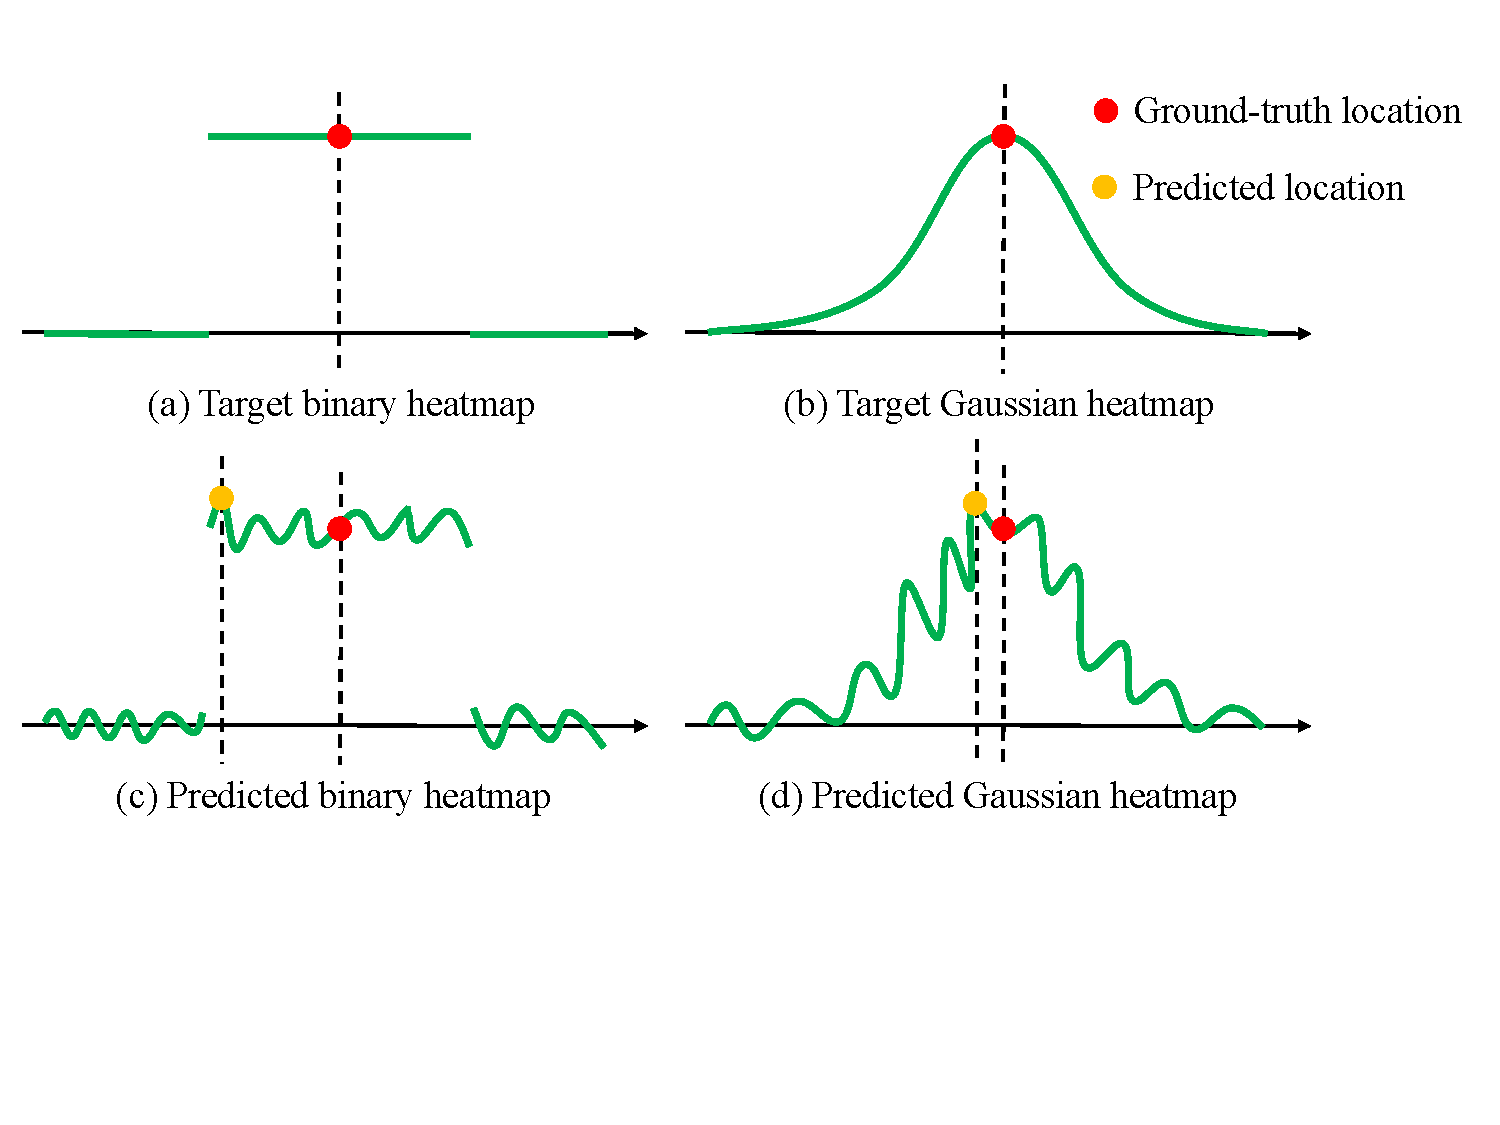
\includegraphics[width=15cm]{multiple_signal_detection/images/heatmap}}
	\caption{Taken from \cite{wang2021lowresolutionhumanposeestimation}}
	\label{}
\end{figure}

\begin{equation}
	H(t) = \max(e^{-\frac{(t-t_1)^2}{2\sigma^2}}, e^{-\frac{(t-t_2)^2}{2\sigma^2}}, \dots)
\end{equation}

\begin{equation}
	p(t) = \begin{cases} 
		e^{H(t)} / \sum_{|t'-x|\lesssim\sigma}e^{H(t')} & |t-x| \lesssim \sigma \\
		0 & \text{else}
	\end{cases} 	% \softmax\{\hat{H}(t') : |t'-x| \lesssim \sigma \}
\end{equation} 
\begin{equation}
	\hat{t} = \sum_t t\,p(t)
\end{equation}
$\hat{y} = \hat{H}(p)$

\begin{equation}
	y(\hat{t}) = \begin{cases}
		1 & \text{$|t-\hat{t}|\leq\sigma$ for any $t$} \\
		0 & \text{else}
	\end{cases}
\end{equation}

\section{CNN and Transformer Models}

\begin{figure}
	\centering
	\makebox[\textwidth]{
		\includegraphics[width=8cm]{multiple_signal_detection/images/heatmap_CNN}
		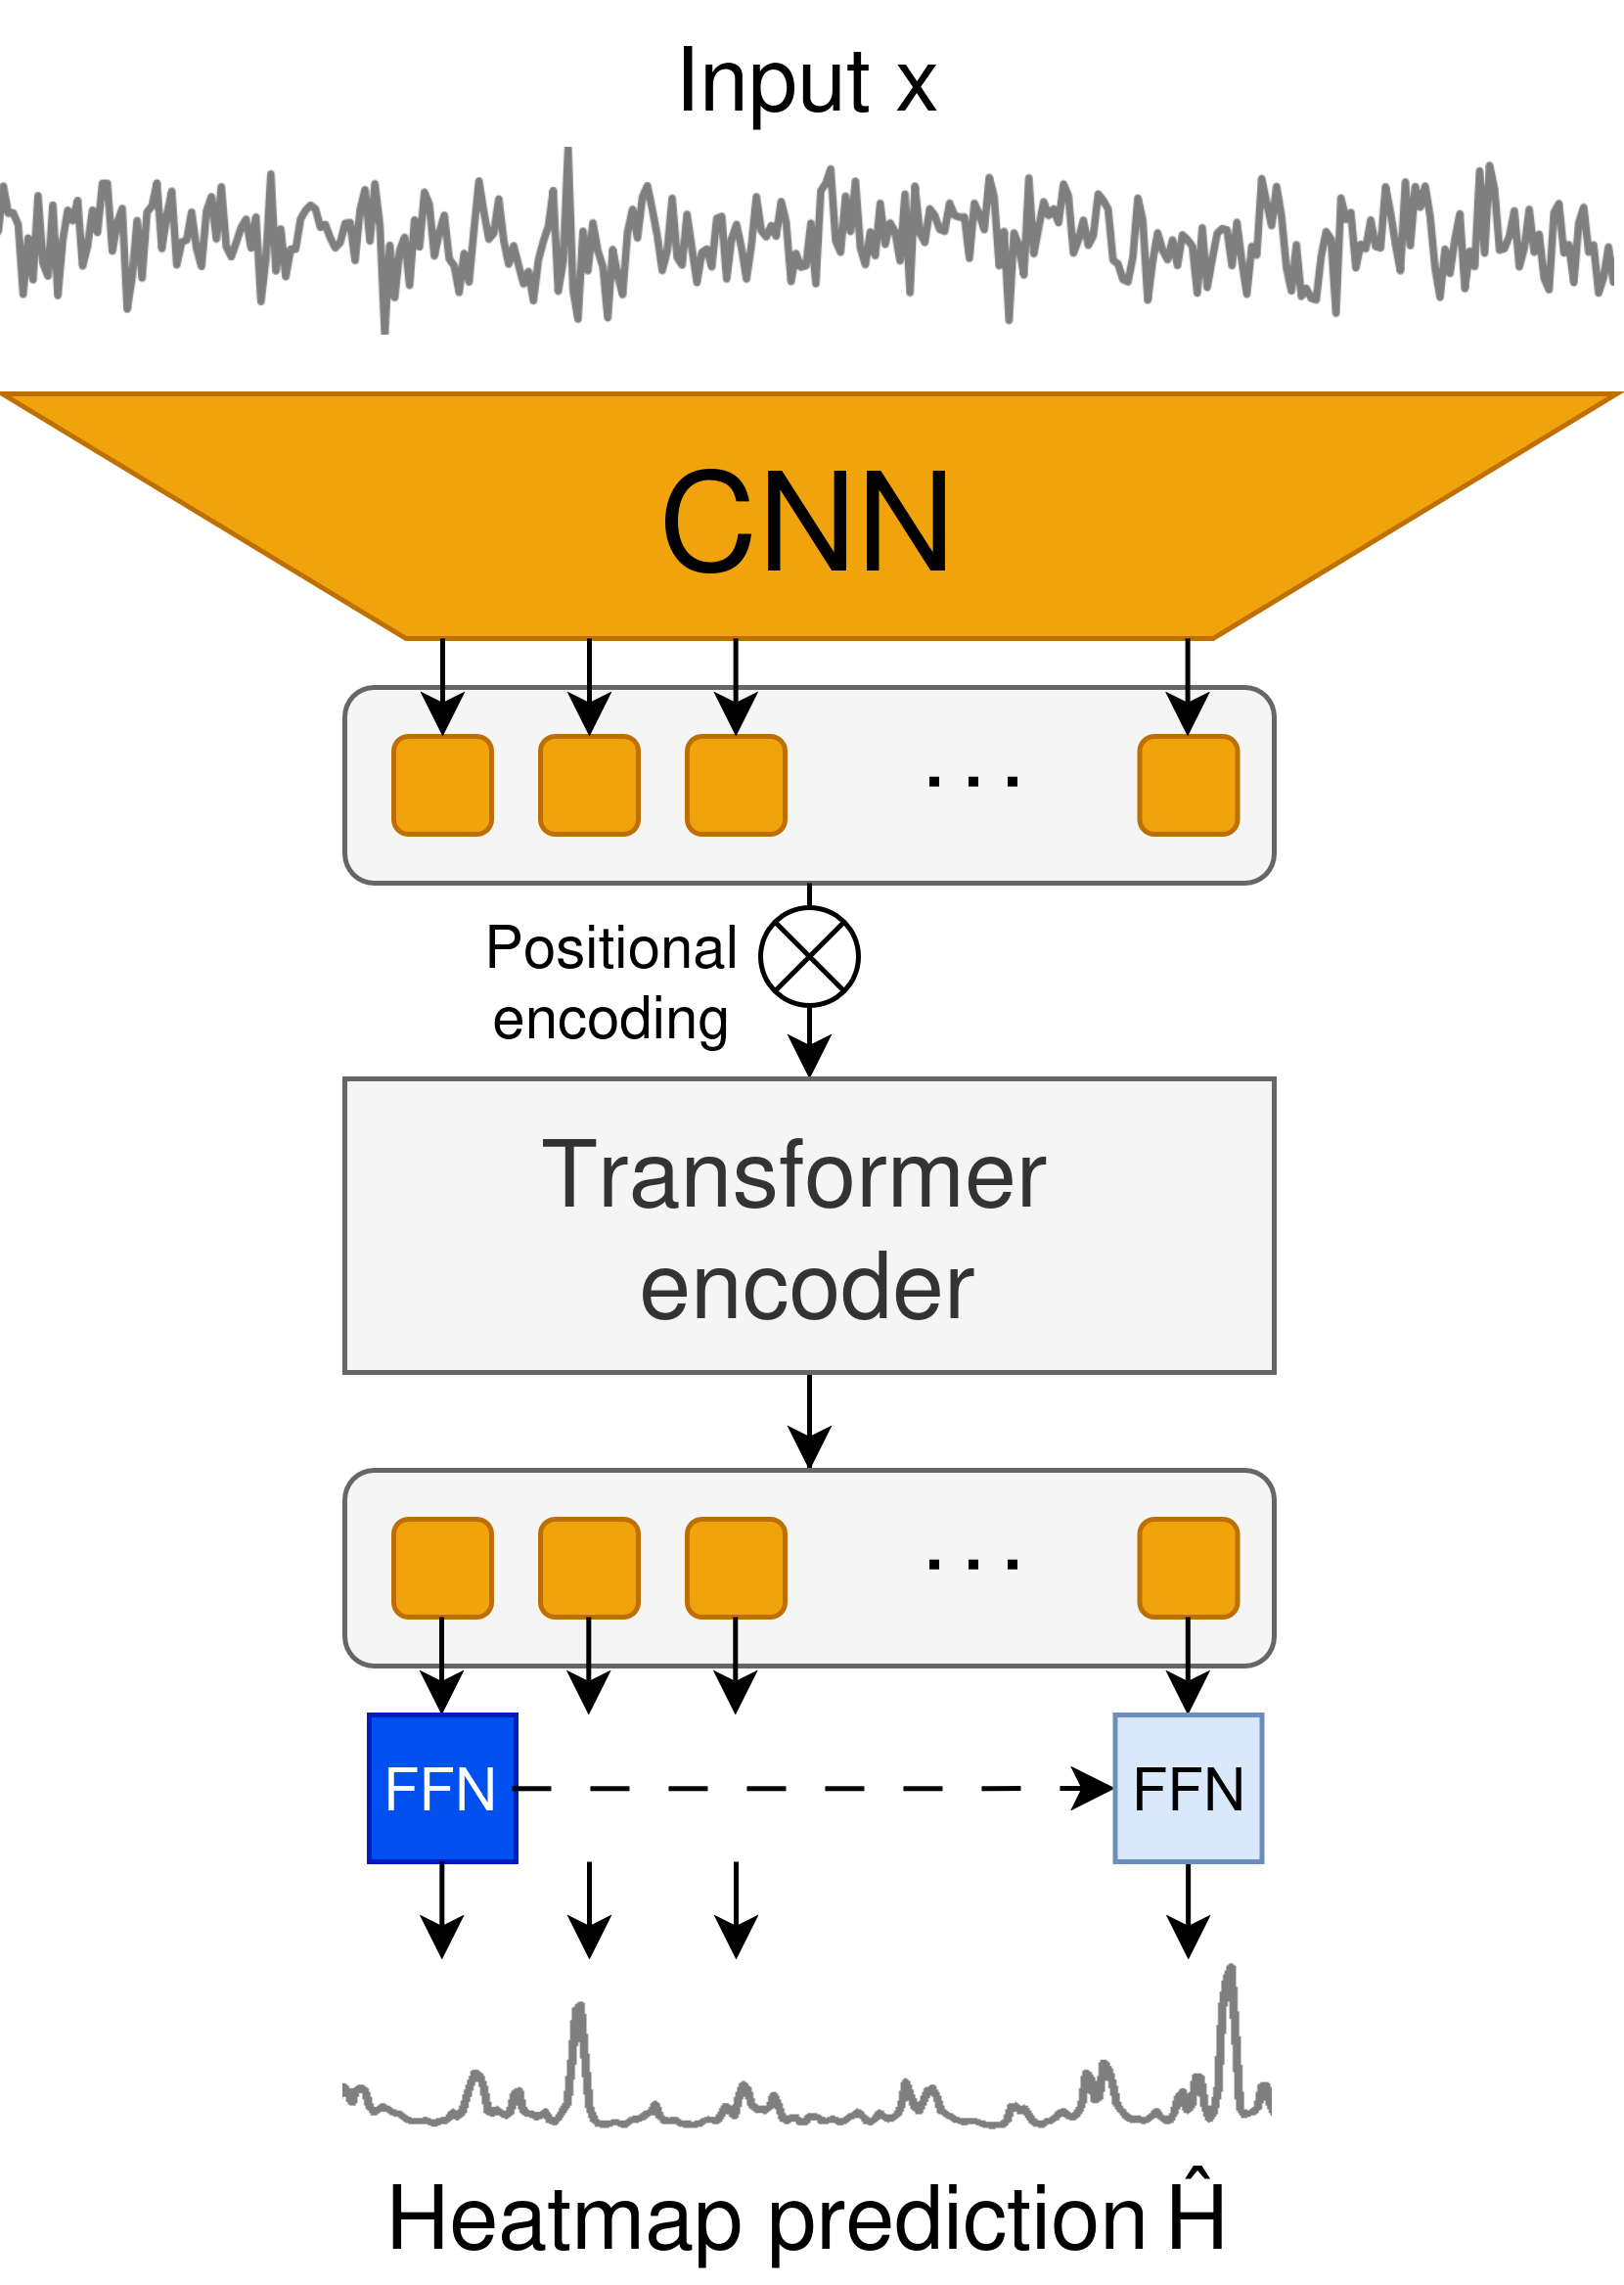
\includegraphics[width=8cm]{multiple_signal_detection/images/heatmap_transformer}
	}
	\caption{}
	\label{}
\end{figure}

\SI{2.2}{\mega\nothing} parameters, \SI{6.7}{\giga\byte}

\begin{equation}
	\pazocal{L}_\text{BCE}(H(t), \hat{H}(t)) = -(\alpha H(t) \ln{\hat{H}(t)} + (1 - \alpha) (1-H(t)) \ln{(1-\hat{H}(t))})
\end{equation}
$\alpha = 0.98$

\begin{figure}
	\centering
	\makebox[\textwidth][c]{%
		\begin{minipage}{9cm}
			\centering
			\makebox[\textwidth]{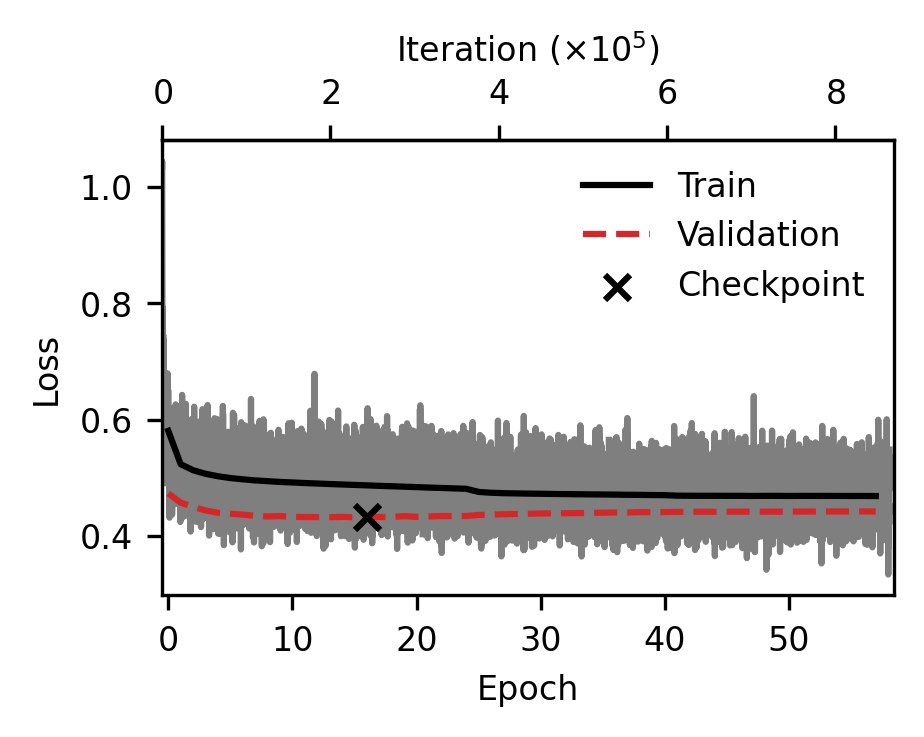
\includegraphics[width=9cm]{multiple_signal_detection/plots/learning_curves/cnn_loss}}
			\captionof{figure}{.}
			\label{fig:heatmap:cnn_learning}
		\end{minipage}%
		\begin{minipage}{9cm}
			\centering
			\makebox[\textwidth]{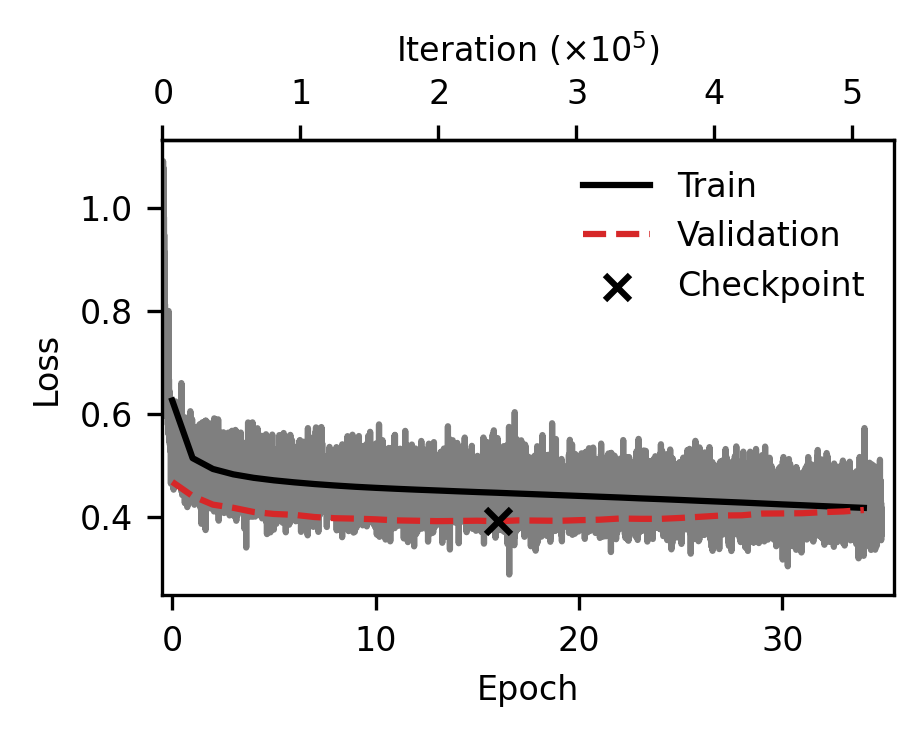
\includegraphics[width=9cm]{multiple_signal_detection/plots/learning_curves/encoder_loss}}
			\captionof{figure}{.}
			\label{fig:heatmap:encoder_learning}
		\end{minipage}
	}
\end{figure}

\section{Performance Comparison}

\begin{figure}
	\centering
	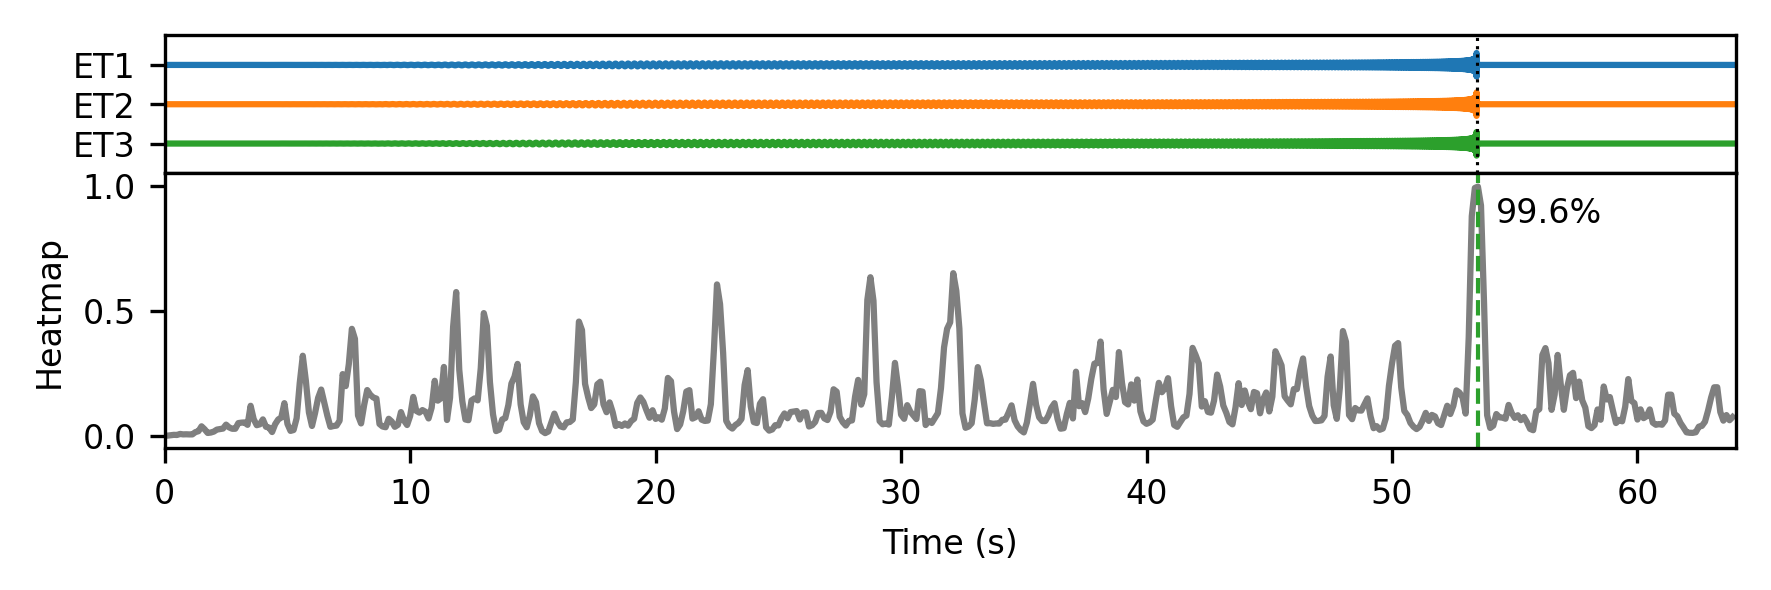
\includegraphics[
	width=15cm,
	trim=0 1cm 0 0,
	clip
	]{multiple_signal_detection/plots/out/300/encoder/1}
	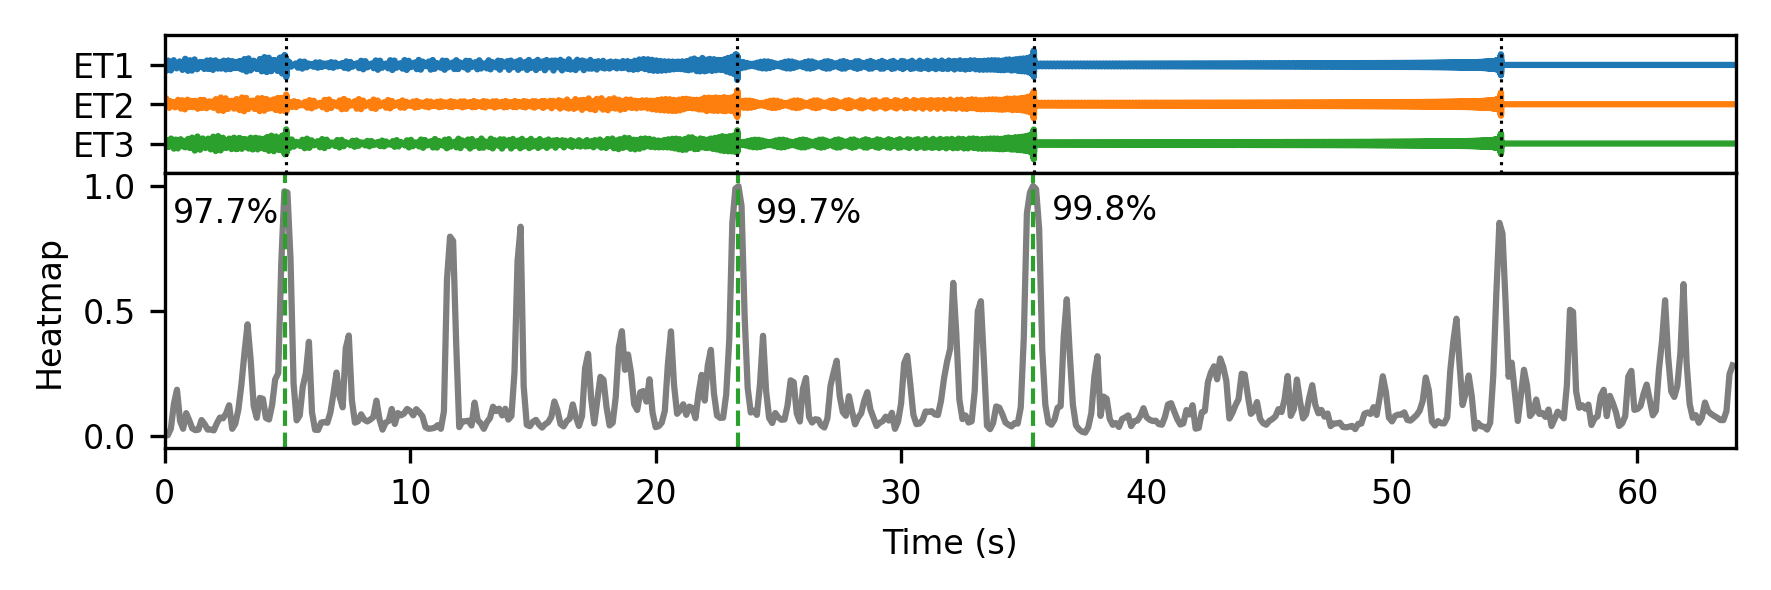
\includegraphics[
	width=15cm,
	trim=0 1cm 0 0,
	clip
	]{multiple_signal_detection/plots/out/300/encoder/5}
	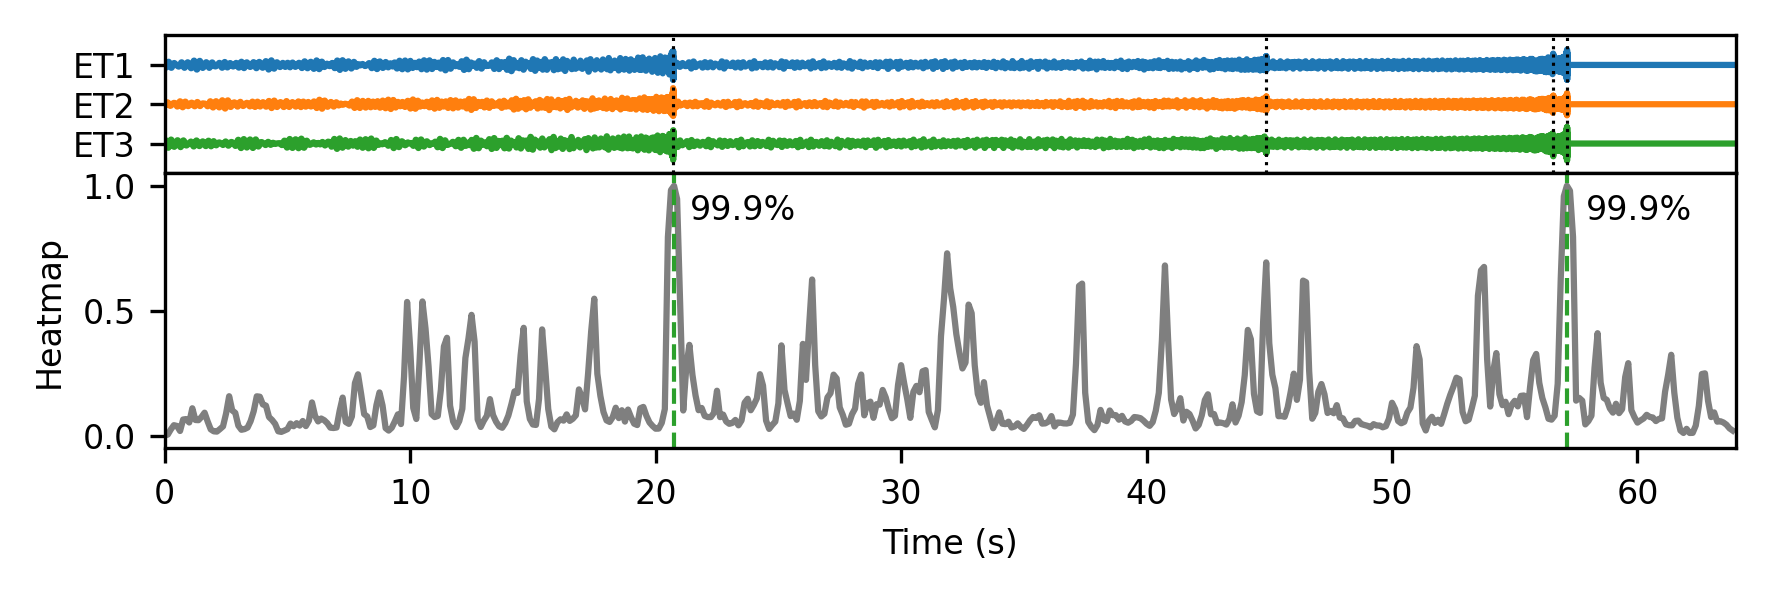
\includegraphics[
	width=15cm,
	trim=0 1cm 0 0,
	clip
	]{multiple_signal_detection/plots/out/300/encoder/10}
	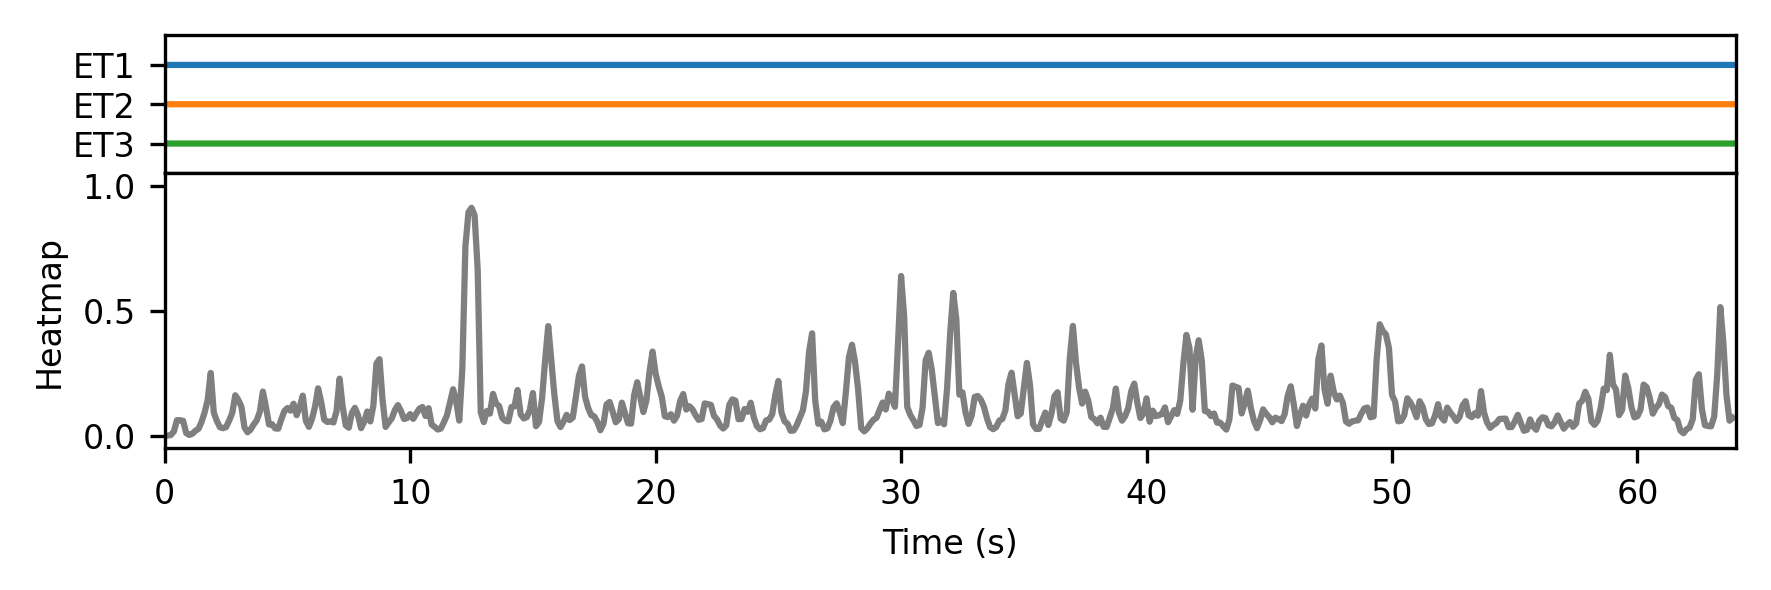
\includegraphics[
	width=15cm,
	trim=0 1cm 0 0,
	clip
	]{multiple_signal_detection/plots/out/300/encoder/11}
	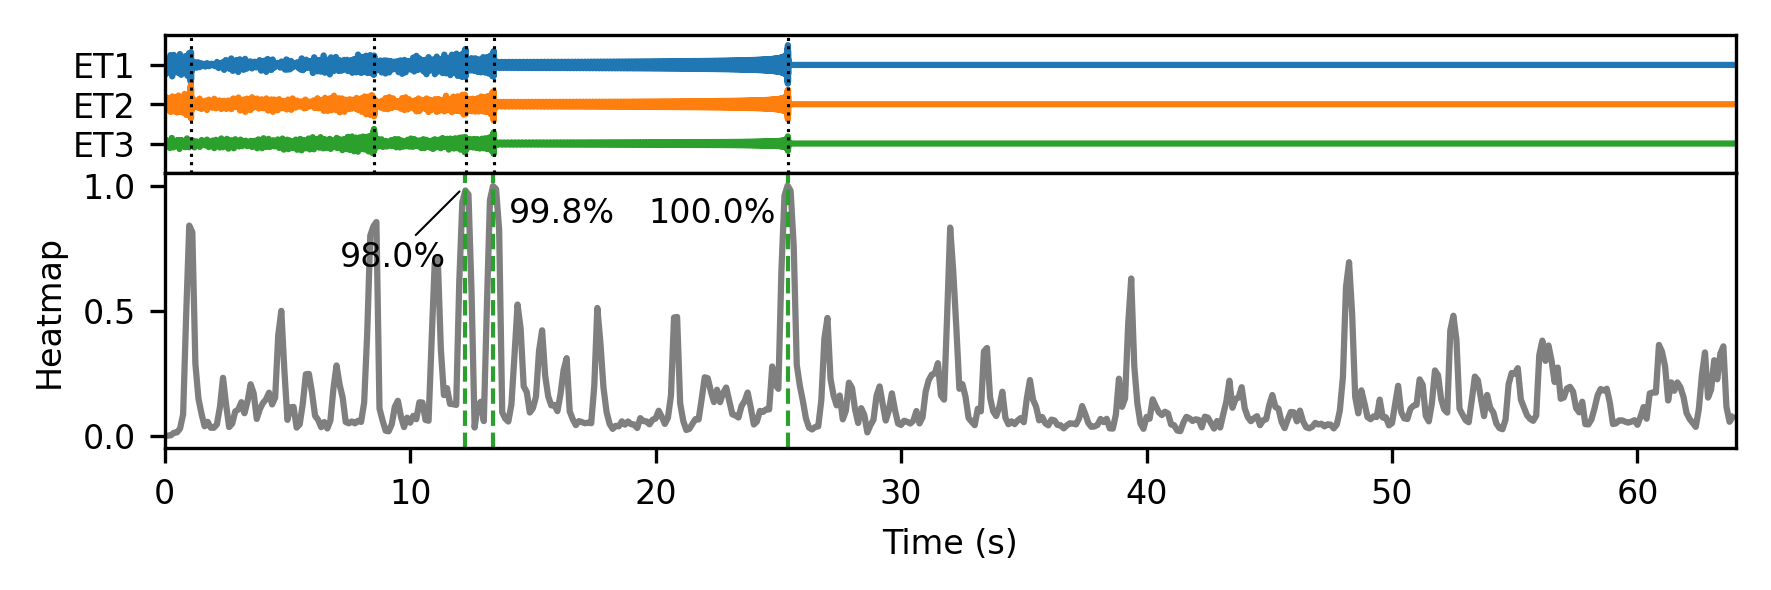
\includegraphics[
	width=15cm,
	]{multiple_signal_detection/plots/out/300/encoder/20}
	\caption{}
	\label{fig:heatmap:encoder_out}
\end{figure}

\begin{figure}
	\centering
	\makebox[\textwidth]{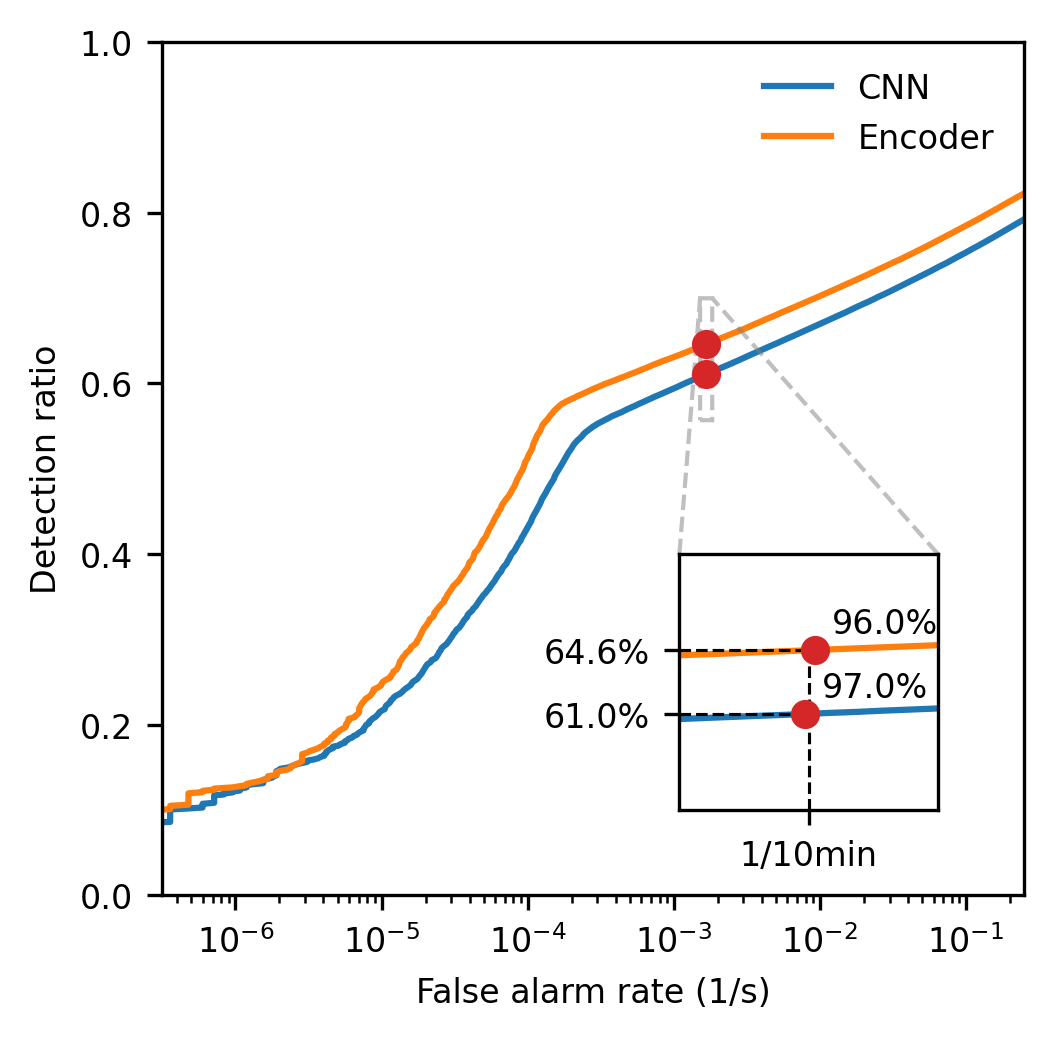
\includegraphics[width=9cm]{multiple_signal_detection/plots/cnn_encoder_far}}
	\caption{}
	\label{fig:heatmap:encoder_far}
\end{figure}

\begin{figure}
	\centering
	\makebox[\textwidth]{\includegraphics[width=12cm]{multiple_signal_detection/plots/num_mergers}}
	\caption{}
	\label{fig:heatmap:num_mergers}
\end{figure}

\section{Injection Study}

\begin{figure}
	\centering
	\makebox[\textwidth]{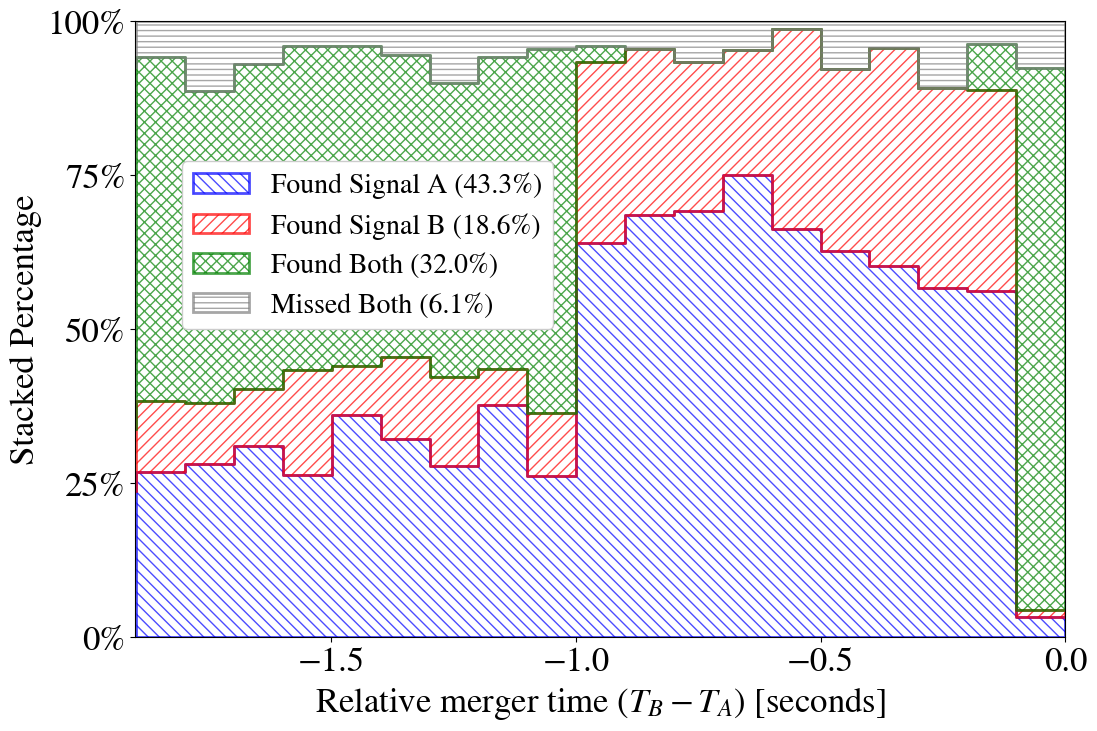
\includegraphics[width=13cm]{multiple_signal_detection/images/delta_tc_stacked_FAR}}
	\captionof{figure}{.}
	\label{fig:heatmap:matched_filtering_deltat}
\end{figure}

\begin{figure}
	\centering
	\makebox[\textwidth]{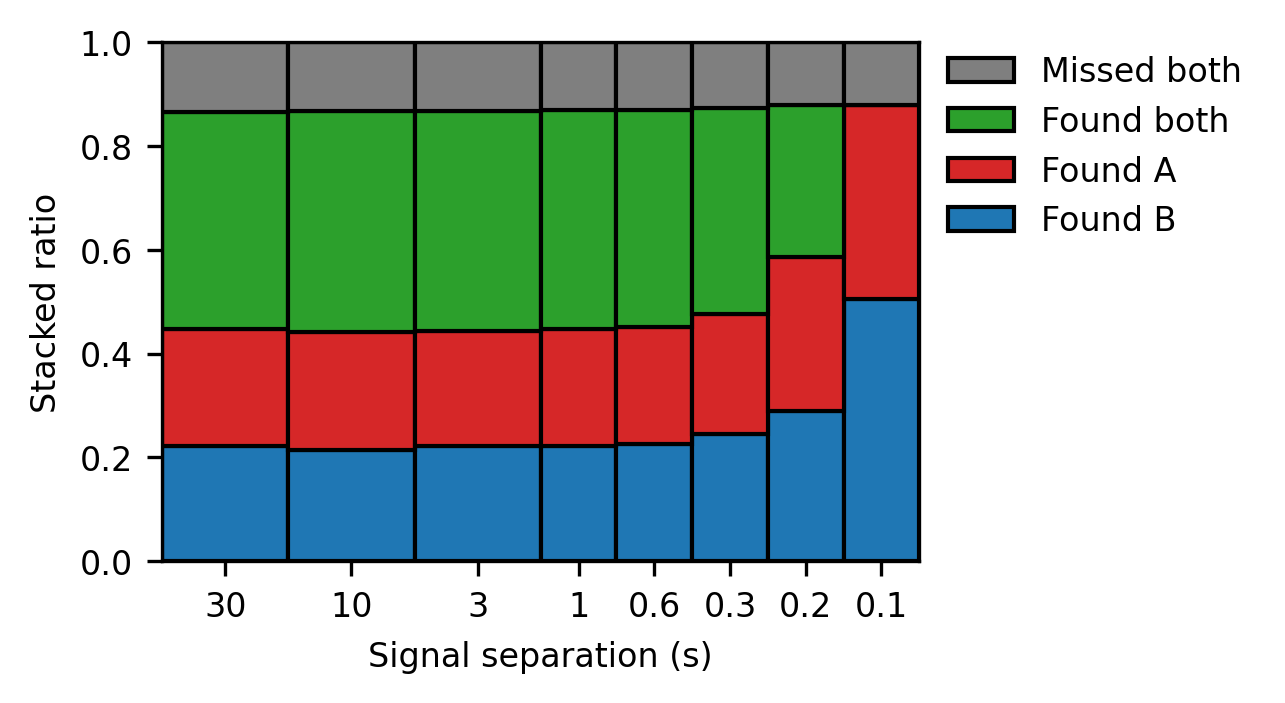
\includegraphics[width=10cm]{multiple_signal_detection/plots/encoder_stacked}}
	\captionof{figure}{.}
	\label{fig:heatmap:enocder_deltat}
\end{figure}

\chapter{Detection Transformer}

\cite{10.1007/978-3-030-58452-8_13}

\section{Architecture and Training}

Ideally, each signal should be assigned exactly one prediction in an optimal manner. These assigned predictions can then labeled based on their class and time values w.r.t.\ the corresponding signal, while all remaining predictions will be labeled false.
To this end, the cost of assigning a prediction $\hat{y}_j$ to a signal with coalescence time $t_i$ is defined as
\begin{equation}
	\pazocal{L}_\text{cost}(t_i, \hat{y}_j) = -\hat{c}_j + \lambda|t_i-\hat{t}_j| \quad \text{with $\lambda = 6$.}
\end{equation}
Let $\tau$ denote an \emph{assignment function} mapping each signal index $i\in I = \{1, 2, \dots, M\}$ to a subset of all prediction indices $j\in J' \subset J = \{1, 2, \dots, N\}$. The \emph{optimal} assignment function $\pi$ will be the realization of $\tau$ that minimizes the total assignment cost over all signals $i$ and corresponding predictions $\tau(i)$:
\begin{equation}
	\pi = \argmin_\tau \sum_{i=1}^M \pazocal{L}_\text{cost}(t_i, \hat{y}_{\tau(i)}).
\end{equation}
This is what is called an \emph{assignment problem} which can be solved with methods implemented by SciPy \cite{2020SciPy-NMeth}. Finally, the ground truth $y_j$ that corresponds to $\hat{y}_j$ can be constructed as
\begin{equation}
	y_j = \begin{cases}
		(1, t_{\pi^{-1}(j)}) & \text{if $j\in J'$ and  $|t_{\pi^{-1}(j)}-\hat{t}_j|\leq\Delta T/2=\SI{0.1}{\second}$} \\
		(0, \varnothing) & \text{else.}
	\end{cases}
\end{equation}
This way, only predictions that are both assigned to a signal and sufficiently close in time are considered true, while all other predictions are treated as false.


\begin{figure}
	\centering
	\makebox[\textwidth]{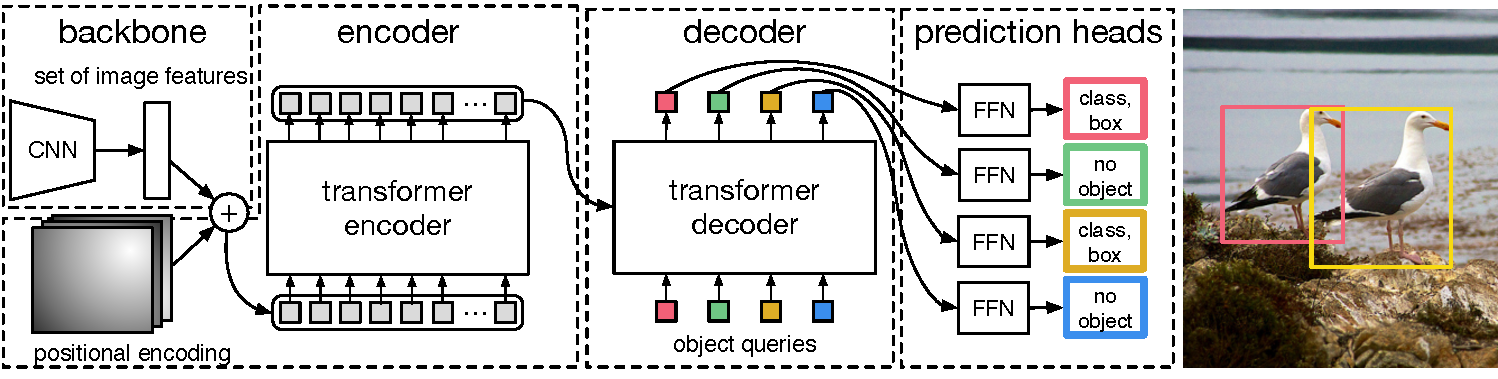
\includegraphics[width=16cm]{multiple_signal_detection/images/DETR_detail_seagulls}}
	\caption{}
	\label{fig:detr:detr}
\end{figure}

\SI{6.2}{\mega\nothing} parameters, \SI{7}{\giga\byte}

\begin{equation}
	\pazocal{L}(y, \hat{y}) = \sum_{i=1}^Q \pazocal{L}_\text{BCE}(c_i, \hat{c}_{\pi(i)}) + \lambda\pazocal{L}_{L_1}(t_i, \hat{t}_{\pi(i)})
\end{equation}
where the BCE loss is unweighted, \emph{i.e.}, $\alpha=1/2,$

% total loss
\begin{figure}
	\centering
	\makebox[\textwidth]{
		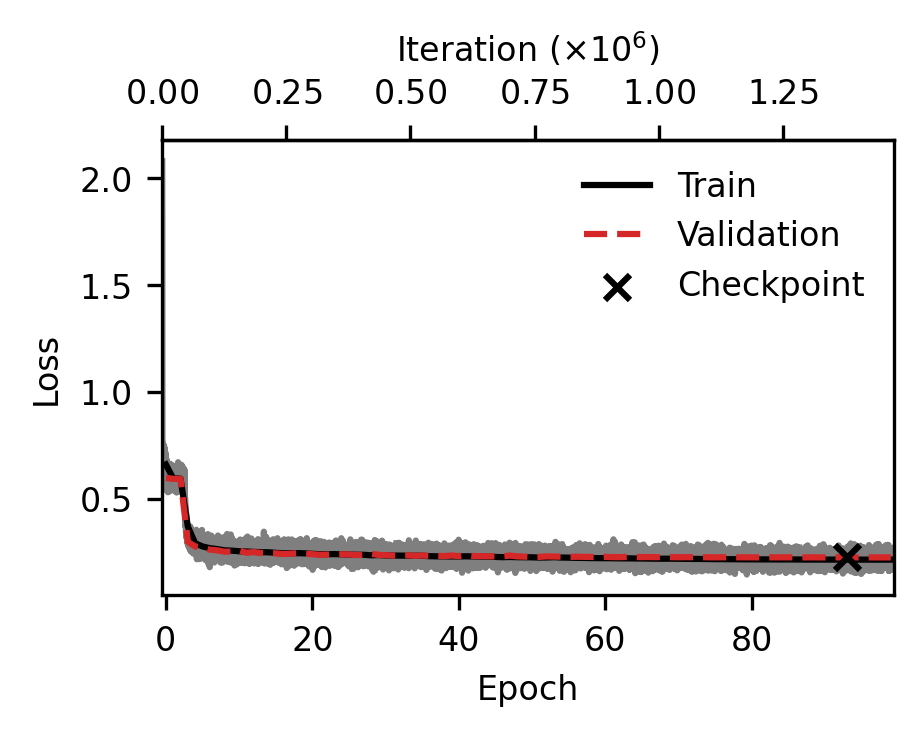
\includegraphics[width=9cm]{multiple_signal_detection/plots/learning_curves/detr_loss}
	}
	\caption{RTX 2080 for \SI{48}{\hour}, Tesla V100 for \SI{48}{\hour}, H200 for \SI{24}{\hour} early stopping after 93th epoch}
	\label{}
\end{figure}

% two losses
\begin{figure}
	\centering
	\makebox[\textwidth]{
		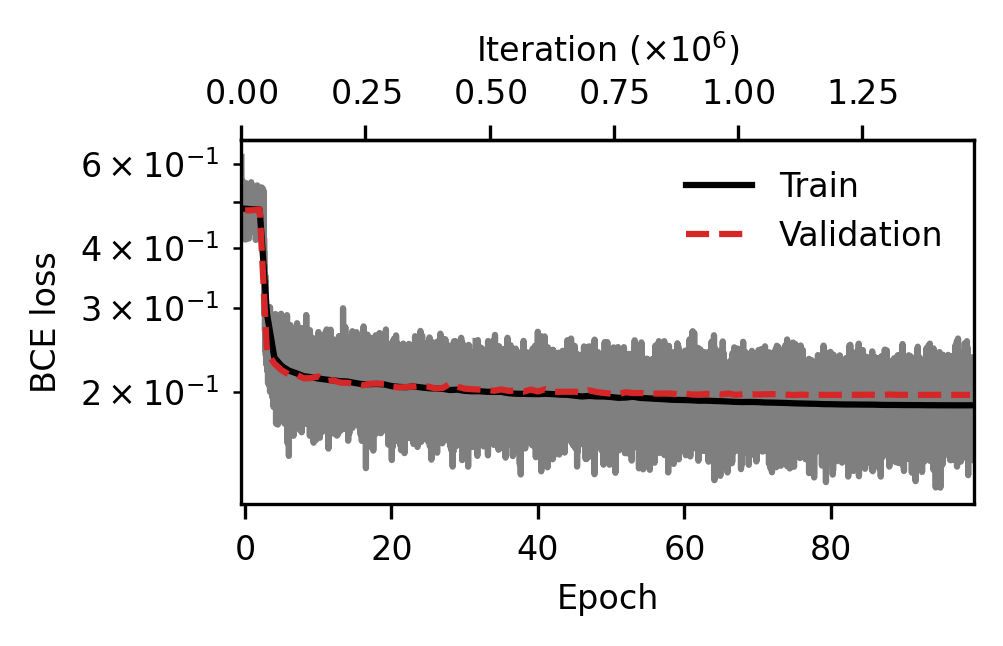
\includegraphics[width=9cm]{multiple_signal_detection/plots/learning_curves/detr_bce_loss}
		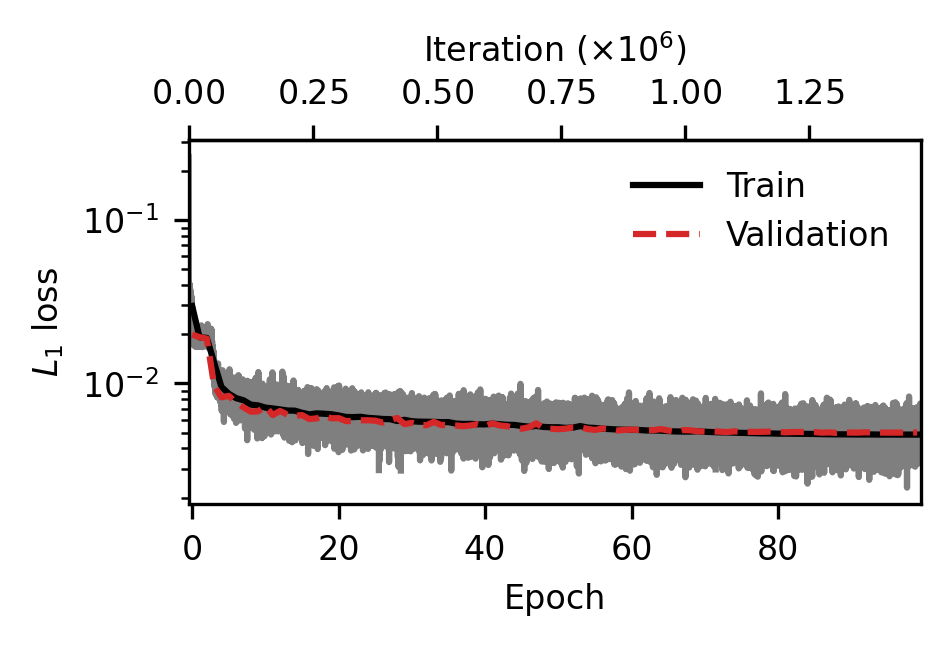
\includegraphics[width=9cm]{multiple_signal_detection/plots/learning_curves/detr_l1_loss}
	}
	\caption{}
	\label{}
\end{figure}

\section{Comparison with Heatmap Regression}

\begin{figure}
	\centering
	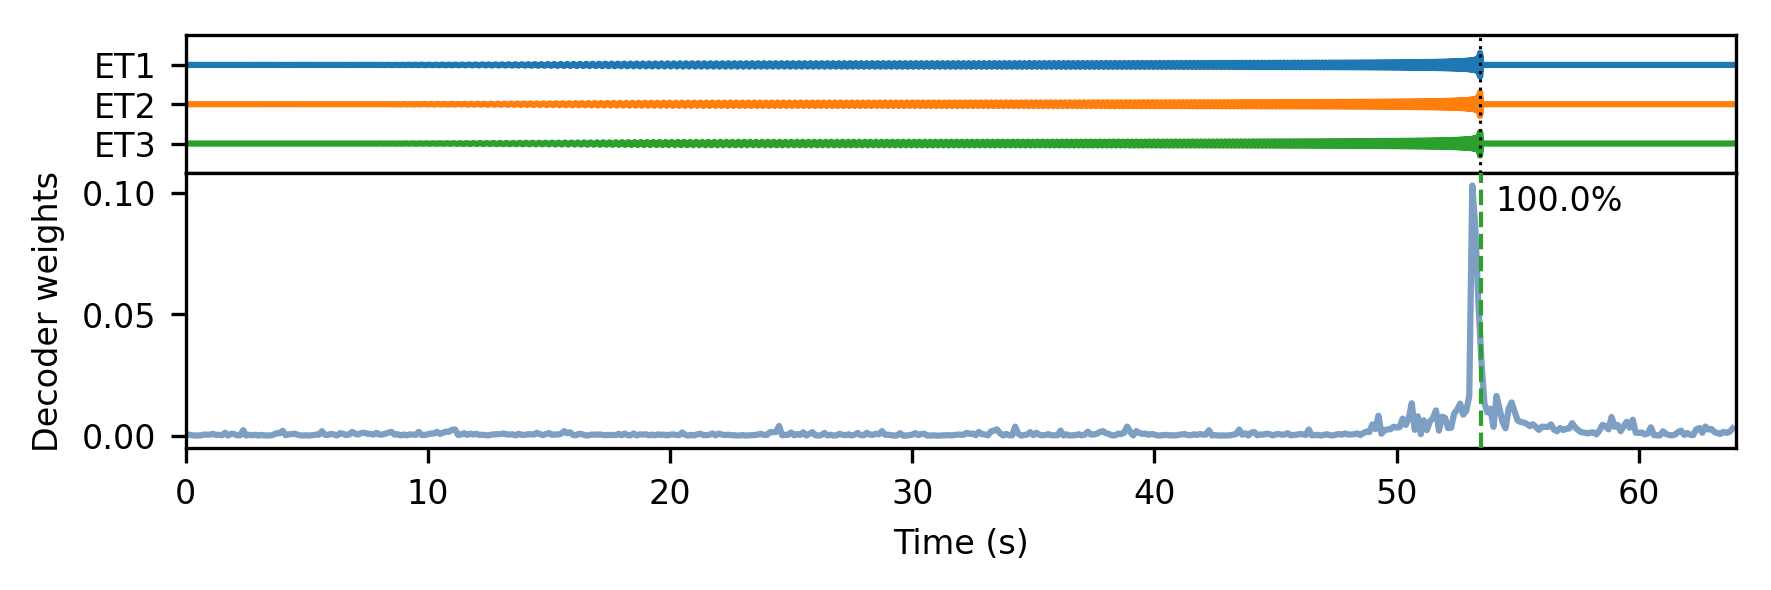
\includegraphics[
	width=15cm,
	trim=0 1cm 0 0,
	clip
	]{multiple_signal_detection/plots/out/300/detr/1}
	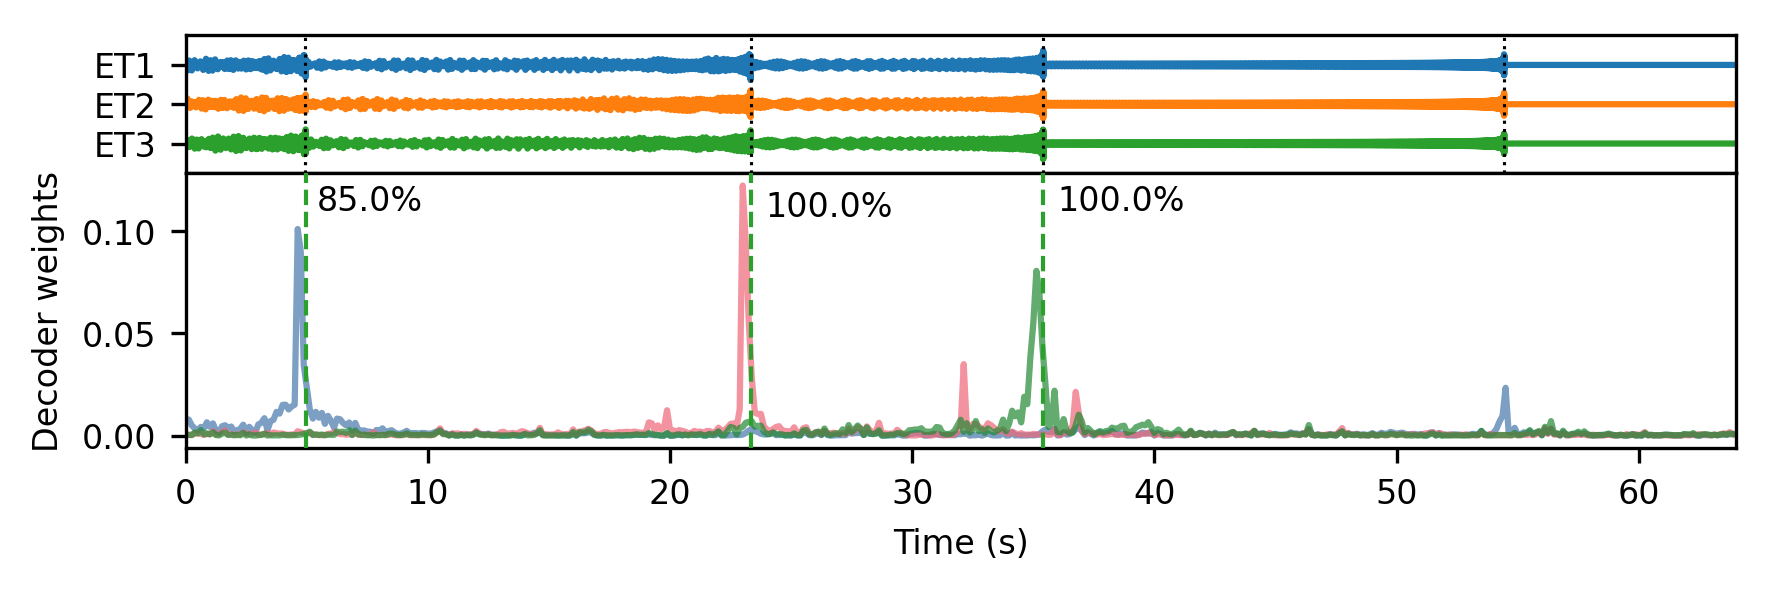
\includegraphics[
	width=15cm,
	trim=0 1cm 0 0,
	clip
	]{multiple_signal_detection/plots/out/300/detr/5}
	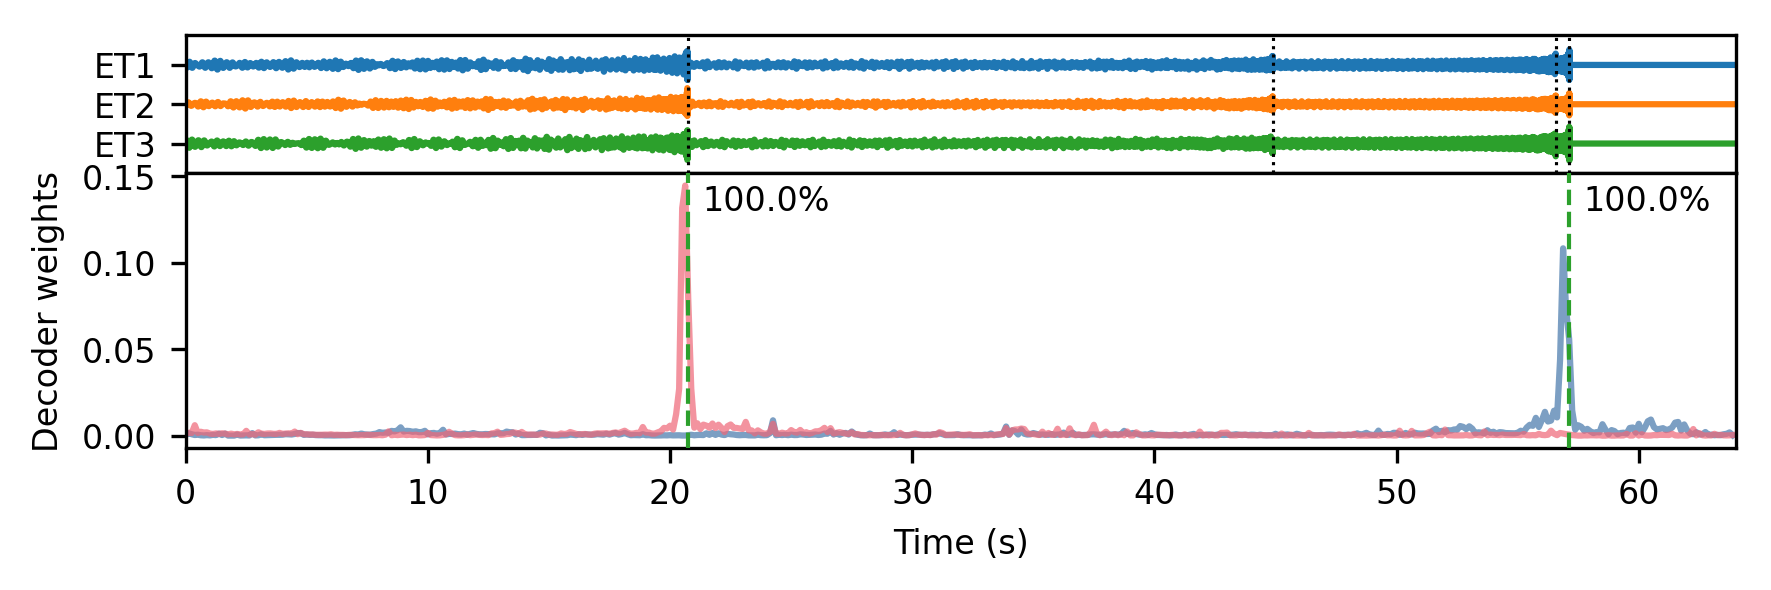
\includegraphics[
	width=15cm,
	trim=0 1cm 0 0,
	clip
	]{multiple_signal_detection/plots/out/300/detr/10}
	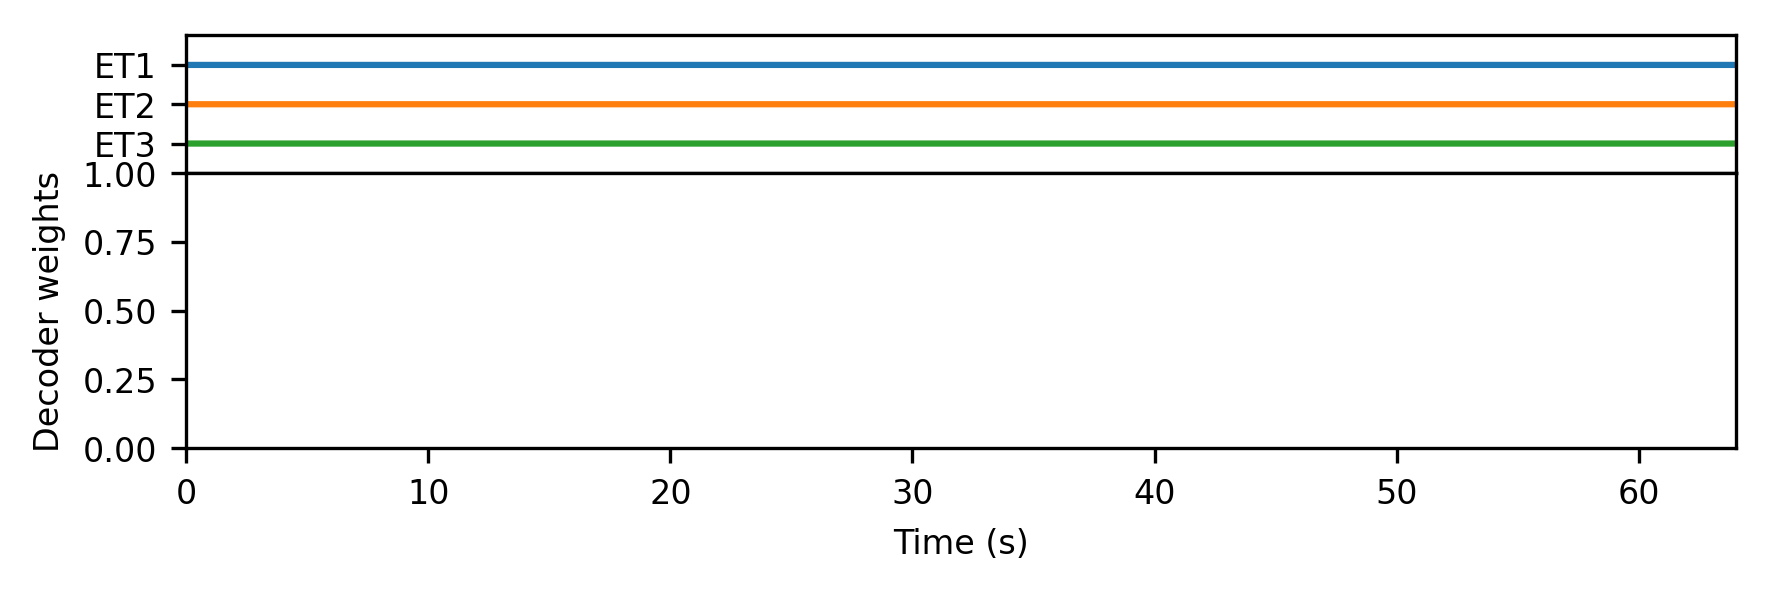
\includegraphics[
	width=15cm,
	trim=0 1cm 0 0,
	clip
	]{multiple_signal_detection/plots/out/300/detr/11}
	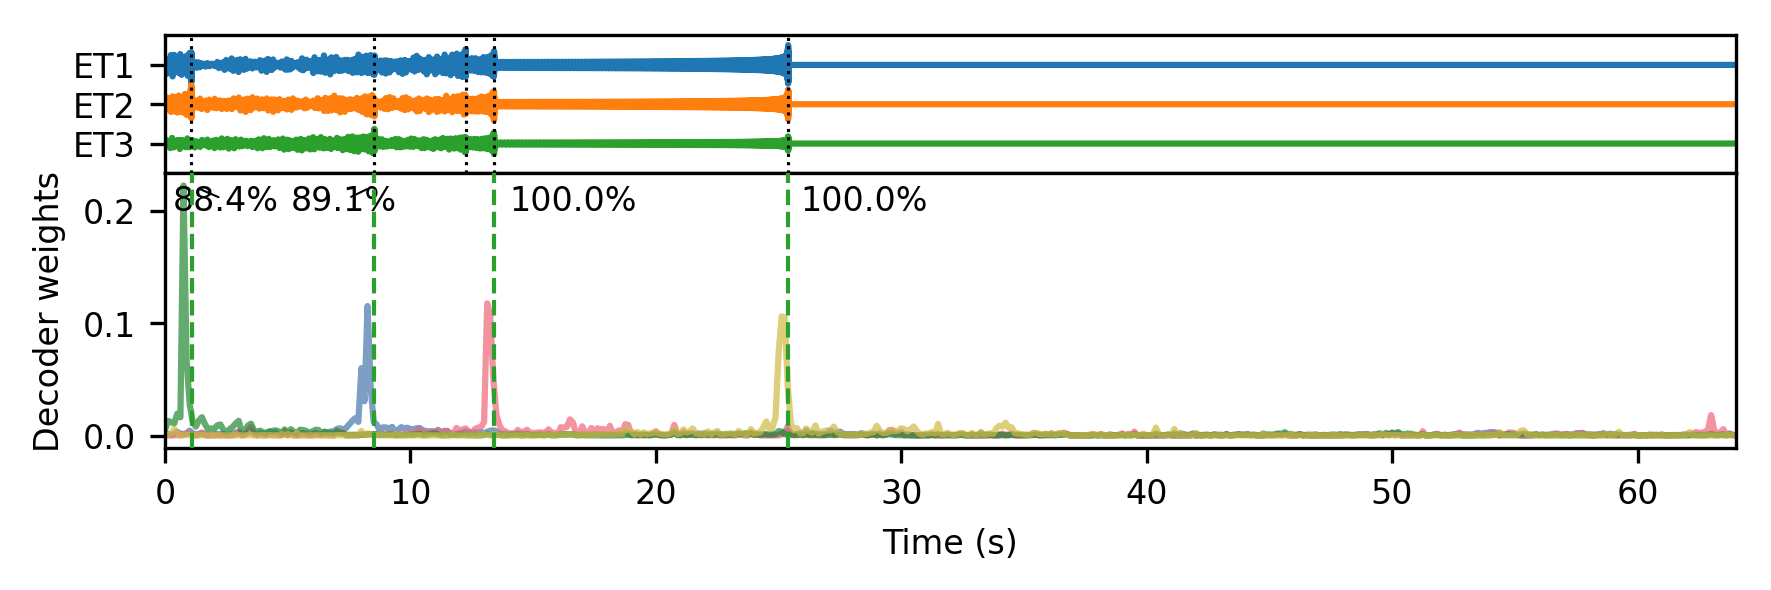
\includegraphics[
	width=15cm,
	]{multiple_signal_detection/plots/out/300/detr/20}
	\caption{}
	\label{fig:heatmap:detr_out}
\end{figure}

\begin{figure}
	\centering
	\makebox[\textwidth]{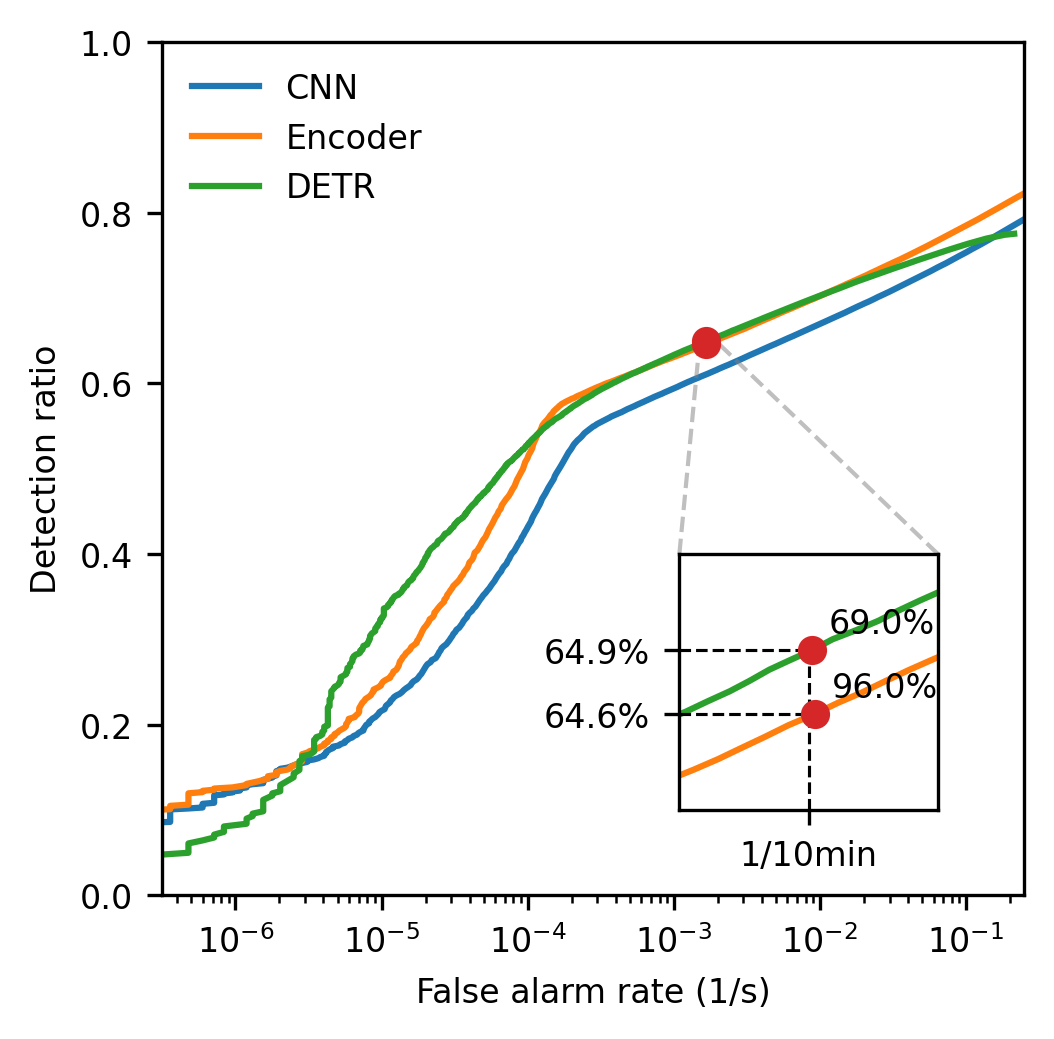
\includegraphics[width=9cm]{multiple_signal_detection/plots/cnn_encoder_detr_far}}
	\caption{}
	\label{fig:detr:far}
\end{figure}

\section{Injection Study}

\begin{figure}
	\centering
	\makebox[\textwidth]{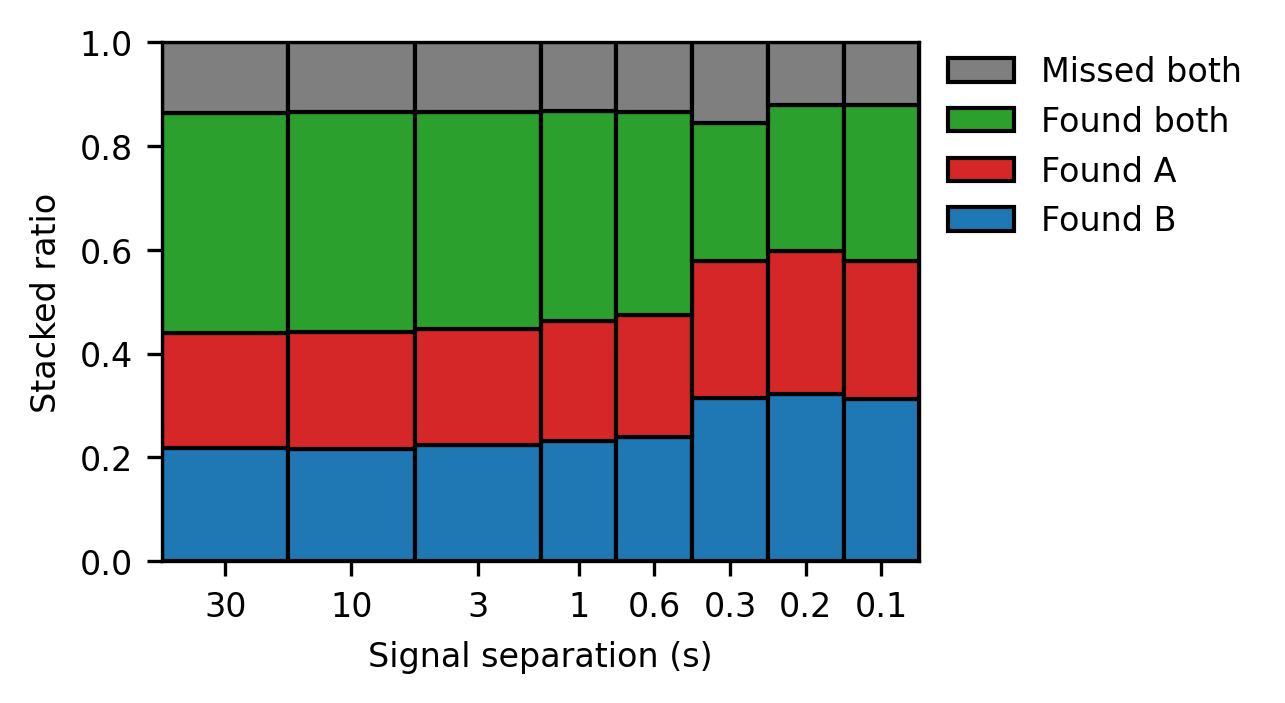
\includegraphics[width=13cm]{multiple_signal_detection/plots/detr_stacked}}
	\captionof{figure}{.}
	\label{fig:heatmap:detr_deltat}
\end{figure}